\documentclass[letterpaper,11pt]{article}
\usepackage[utf8x]{inputenc}
\usepackage{enumerate}
\usepackage{enumitem}
\usepackage{fullpage}
\usepackage{amsmath}

\usepackage{pgf}
\usepackage{tikz}
\usetikzlibrary{arrows,shapes,trees}

%opening
\title{Physics 601 (Fall 2012) \\ Homework Assignment 2: Solutions}
\date{Due: Thursday September 13, 2012}

\begin{document}

\maketitle

\paragraph*{Generalized Coordinates and the Lagrange's Equations}
\begin{enumerate}
 \item A particle of charge $e$ in an electromagnetic field sees a generalized potential $U(\vec{r},\vec{v},t) = e \phi - e \vec{v} \cdot \vec{A}$.  Show that under the gauge transformation
  \begin{eqnarray*}
   \vec{A'} & = & \vec{A} + \vec{\nabla} \psi(\vec{r},t) \\
   \phi'    & = & \phi - \frac{\partial\psi(\vec{r},t)}{\partial t}
  \end{eqnarray*}
 the Lagrangian changes only by a total time-derivative $\frac{dF}{dt}$ for some function $F(\vec{r},t)$.
\end{enumerate}
We can write the Lagrangian with the generalized potential as $L = T - U = T - e \phi + e \vec{v} \cdot \vec{A}$.  Under the given transformation this becomes
\begin{eqnarray*}
 L' & = & T - e \phi' + e \vec{v} \cdot \vec{A'} \\
 & = &  - e \phi + e \frac{\partial\psi}{\partial t} + e \vec{v} \cdot \vec{A} + e \vec{v} \cdot \vec{\nabla} \psi \\
 & = & L + e \frac{\partial\psi}{\partial t} + e \vec{v} \cdot \vec{\nabla} \psi \\
 & = & L + e \frac{d\psi}{dt},
\end{eqnarray*}
where we used that
\begin{equation*}
 \frac{d\psi}{dt} = \sum_i \frac{\partial\psi}{\partial x_i} \dot{x}_i + \frac{\partial\psi}{\partial t} = \vec{v} \cdot \vec{\nabla} \psi + \frac{\partial\psi}{\partial t}.
\end{equation*}

\begin{enumerate}[resume]
 \item A block of mass $m$ slides without friction down a wedge of mass $M$, which is free to slide without friction on a horizontal table.
 \begin{enumerate}
  \item Determine the Lagrangian for the system, using $q_1$ and $q_2$ as generalized coordinates.
  \item Determine the equations of motion.
  \item Let $\ell$ be the length of the sloping face of the wedge.  How long does it take the block to reach the table, assuming the entire system starts from rest with $q_1 = 0$?
 \end{enumerate}
 \textit{Note: This problem was part of the qualifying exam in August 2011.}
 \begin{center}
  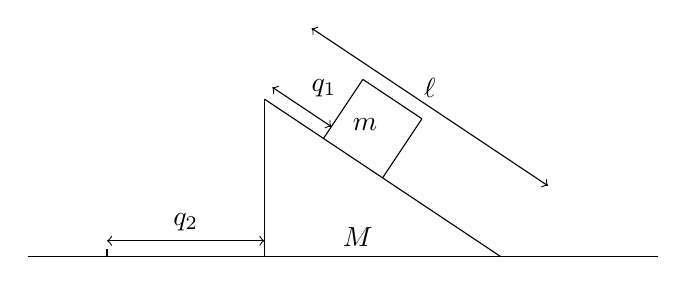
\begin{tikzpicture}
   % X axis
   \draw (-4,-0) -- (4,-0);
   \draw (-3,-0) -- (-3,0.1);
   % Wedge
   \draw (-1,0) -- (-1,2);
   \draw (-1,2) -- (2,0);
   \draw (-1,0) -- node[above left]{$M$} (2,0);
   \draw[<->] (-0.4,2.9) -- node[above]{$\ell$} (2.6,0.9);
   \draw[<->] (-3,0.2) -- node[above]{$q_2$} (-1,0.2);
   % Block
   \draw (-0.25,1.5) -- node[below right]{$m$} (0.25,2.25);
   \draw (0.25,2.25) -- (1,1.75);
   \draw (0.5,1) -- (1,1.75);
   \draw[<->] (-0.9,2.15) -- node[above right]{$q_1$} (-0.15,1.65);
  \end{tikzpicture}
 \end{center}
\end{enumerate}
The kinetic and potential energy can be written as
\begin{eqnarray*}
 T & = & \frac{1}{2} M \dot{q}_2^2 + \frac{1}{2} m \left( (\dot{q}_2 + \dot{q}_1\cos\alpha)^2 + \dot{q}_1^2 \sin^2\alpha \right), \\
 V & = & - m g q_1 \sin\alpha, \\
 L & = & \frac{1}{2} M \dot{q}_2^2 + \frac{1}{2} m \left( (\dot{q}_2 + \dot{q}_1\cos\alpha)^2 + \dot{q}_1^2 \sin^2\alpha \right) + m g q_1 \sin\alpha.
\end{eqnarray*}
The equations of motion are
\begin{eqnarray*}
 m\ddot{q}_1 + m\ddot{q}_2 \cos\alpha - mg \sin\alpha & = & 0, \\
 (M + m) \ddot{q}_2 + m\ddot{q}_1 \cos\alpha & = & 0.
\end{eqnarray*}
We can solve for $\ddot{q}_2$ using the second equation and find
\begin{eqnarray*}
 & & \ddot{q}_2 = \frac{m}{M + m} \ddot{q}_1 \cos\alpha, \\
 & & \ddot{q}_1 + \frac{m}{M + m} \cos^2\alpha = mg \sin\alpha.
\end{eqnarray*}
Integration with the given initial conditions on $q_1$ then gives
\begin{equation*}
 q_1 = \frac{1}{2} \frac{\sin\alpha}{1 - \frac{m}{M + m} \cos^2\alpha} g t^2,
\end{equation*}
or inversely
\begin{equation*}
 t = \sqrt{\frac{2\ell}{g} \frac{1 - \frac{m}{M + m} \cos^2\alpha}{\sin\alpha}}.
\end{equation*}

\begin{enumerate}[resume]
 \item A system of three masses is arranged on the corners of a foldable frame with length $a$ (\textit{i.e.} the mass $m_2$ can move along the vertical axis as $\theta$ changes).  The whole system is rotating about the vertical axis with angle $\phi$.  Determine the Lagrangian as a function of $\phi$ and $\theta$.  From the equations of motion determine the equilibrium angle for given $\dot\phi = \omega$.
 \begin{center}
  \begin{tikzpicture}
   % Axis
   \draw (0,-3) -- (0,3);
   % Frame
   \draw (0,+2.5) -- node[above right]{$a$} (+2,0) node[right]{$m_1$};
   \draw (0,+2.5) -- node[above left]{$a$} (-2,0) node[left]{$m_1$};
   \draw (+2,0) -- node[below right]{$a$} (0,-2.5) node[below left]{$m_2$};
   \draw (-2,0) -- node[below left]{$a$} (0,-2.5);
   % Angle
   \draw (0,1.5) node[below right]{$\theta$} arc (-90:-51:1);
  \end{tikzpicture}
 \end{center}
\end{enumerate}
The potential energy is
\begin{equation*}
 V = 2 m_1 g a \cos\theta + 2 m_2 g a \cos\theta = 2 (m_1 + m_2) g a \cos\theta.
\end{equation*}
The velocities are
\begin{eqnarray*}
 v_1^2 & = & a^2\dot\theta^2 + a^2\dot\phi^2\sin^2\theta, \\
 v_2^2 & = & 2 a^2 \dot\theta^2 \sin^2\theta.
\end{eqnarray*}
The kinetic energy is then
\begin{equation*}
 T = m_1 a^2 (\dot\theta^2 + \dot\phi^2 \sin^2\theta) + m_2 a^2 \dot\theta^2 \sin^2\theta.
\end{equation*}
The Lagrangian is then
\begin{equation*}
 L = m_1 a^2 (\dot\theta^2 + \dot\phi^2 \sin^2\theta) + m_2 a^2 \dot\theta^2 \sin^2\theta - 2 (m_1 + m_2) g a \cos\theta.
\end{equation*}
We could write the full equation of motion for $\theta$ but all terms in $\frac{\partial L}{\partial \dot\theta}$ will have at least a $\dot\theta$ and will be zero in equilibrium.  Therefore we only need $\frac{\partial L}{\partial \theta}$.  In equilibrium the equation of motion the becomes
\begin{equation*}
 \frac{\partial L}{\partial \theta}\Big|_{\dot\theta = 0, \dot\phi = \omega} = 2 m_1 a^2 \omega^2 \sin\theta\cos\theta - 2 (m_1 + m_2) g a \sin\theta = 0.
\end{equation*}
The equilibrium angle is then
\begin{equation*}
 \cos\theta = \frac{1}{\omega^2} \frac{g}{a} \frac{m_1+m_2}{m_1}.
\end{equation*}

\end{document}
